\documentclass[UTF8,a4paper,12pt]{ctexart}

%---preamble---
%dependency package
\usepackage{amsmath}
\usepackage{amssymb}
\usepackage[colorlinks=false]{hyperref}
\usepackage{setspace}
\usepackage{enumerate}
\usepackage{cases}
\usepackage{tikz}
\usepackage{tikz-3dplot}
\usepackage{caption}
\usepackage{subcaption}
\usepackage{lmodern}
\usepackage{siunitx}
\usepackage[T1]{fontenc}
\usepackage[parfill]{parskip}
\usepackage[toc, page]{appendix} 
\usepackage{color}
\usepackage[most]{tcolorbox}
\usepackage{etoolbox}
\usepackage[intoc]{nomencl}
\usepackage{booktabs}


%\newcommand{\myfront}{\textbf{\texfsf{Fancy Text}}}


\title{Awakenlion controller}
\author{金花}
\date{\today}
\pagestyle{empty}



%正文区(文稿区)
\begin{document}
%---Style Setting---
\ctexset { 
    section={
     titleformat=\raggedright,
     name=\S
     },
     subsection={
     titleformat=\raggedright
     },
     subsubsection={
     titleformat=\raggedright
     }
}
\newtcolorbox{notitlebox}[2][]
     {
    colback=blue!5!white,colframe=blue!75!black,breakable
    }
\newtcolorbox{titlebox}[2][]
    {
    colback=green!6!white,colframe=green!65!black,
     fonttitle=\bfseries,coltitle=white,                            colbacktitle=green!65!black,
        title=#2,#1,attach boxed title to top center={yshift=-2mm},enhanced,breakable
     }
\linespread{1.35}
\setstretch{1.523}

  \maketitle

  % \begin{titlebox}{什么是系统?}

  % \end{titlebox}

%------------------------------------

%----------流程框图------------------
% \tikzstyle{startstop} = [rectangle, rounded corners, minimum width=3cm, minimum height=1cm,text centered, draw=black, fill=red!30]
% \tikzstyle{process} = [rectangle, minimum width=3cm, minimum height=1cm, text centered, draw=black, fill=orange!30]
% \tikzstyle{decision} = [diamond, minimum width=3cm, minimum height=1cm, text centered, draw=black, fill=yellow!30]
% \tikzstyle{arrow} = [thick,->,>=stealth]


\tikzstyle{startstop} = [  minimum width=2.5cm, minimum height=0.8cm,text centered]
\tikzstyle{process} = [ minimum width=2.5cm, minimum height=0.8cm, text centered,]
\tikzstyle{sys} = [rectangle, minimum width=2.5cm, minimum height=0.8cm, text centered, draw=black]
\tikzstyle{arrow} = [thick,->,>=stealth]







  \begin{center}
    \tableofcontents
  \end{center}
  \newpage

  \section{引言}
  \begin{flushleft}
    \hspace{2em}此文档的初衷是让大家轻松地入门电控代码的控制器,缩短大家从理论到实践的时间。文档将会结合信号与系统和自动控制原理的相关知识,为大家讲解我们战队所需要的控制器,以及如何设计控制器。如果觉得作者本人写的不够详细或者有失偏颇,本人会在每一个知识点的后面附带上我学习过的网址,大家可以搜索着来学习。
    \par\hspace{2em}本文档还会手把手教你如何操作,即使不看理论知识也可以按照步骤来直接得到结果。


  \end{flushleft}
  \section{理论知识}

  \begin{flushleft}
    以下是设计一个控制器所需要用到的理论知识,知识深度仅停留在工程应用的层面,不需要深究其数学原理,但是想要看懂还是需要基本的高数知识。以下的知识只需要将他们看作工具就好了,我们最终的目的就是得到传递函数,依据传递函数来设计所需要的控制器。我尽量会以是什么,怎么用的框架来解释下面的知识,其更深层的含义我会附上链接。
  \end{flushleft}

  \subsection{线性时不变系统(LTI)}
    \begin{flushleft}
      为什么我们要先讲线性时不变系统呢?因为我们战队的代码所设计和分析的控制器都是基于线性时不变系统来研究的。
      \par 实际上线性时不变系统是一个理想化的数学模型,在生活中基本不存在完全符合线性时不变系统定义的系统。主要是以下两个原因:
      \begin{notitlebox}
          \par1.线性系统的限制:
          \begin{itemize} 
            \item 许多系统在小信号范围内表现出线性特性,但在大信号条件下会出现非线性失真,如放大器在信号过强时的饱和现象。
            \item 机械系统如弹簧-质量系统在小振幅下可近似为线性,但超过弹性限度时会表现出非线性行为
          \end{itemize}

          \par2.时不变性的挑战:
          \begin{itemize} 
          \item 理想的时不变系统要求其参数不随时间变化,但在现实中,环境因素如温度、湿度可能影响系统参数,导致时变性。
          \item 电子元件可能因老化或温度变化而改变特性,从而引入时变性。  
          \end{itemize}
          \begin{flushleft}
           但因为LTI模型简单易于处理,其分析方法(如傅里叶变换、拉普拉斯变换、卷积等)是通用的,所以我们会在一定合理的范围和时间内,将系统近似为LTI系统。\par 即使是遇到完全是非线性和时不变的系统我们都会尽量将其线性化(如工作点线性化、分段近似等)和时不变近似(如慢变参数近似、时间平均化等),以此来简化我们的分析。
          \end{flushleft}
      \end{notitlebox}
    \end{flushleft}
    \begin{flushleft}
      OK,了解完上面的原因后,我们来真正的开始学线性时不变系统。
    \end{flushleft}
    \subsubsection{系统}
    \begin{titlebox}{什么是系统?}
      \begin{flushleft}
        
        \par 系统是指若干关联的事物组合而成具有特定功能的整体,系统可以是我们的云台,可以是一个电机,也可以是一个底盘。
        \par 系统的作用: 对输入信号进行加工和处理,将其转换为输出信号
        \par 表示如下:
        \begin{tikzpicture}[node distance=5cm]
          
          \node (start) [startstop] {输入信号(激励)};
          \node(input)[sys,right of=start]{系统};
          \node (output) [process, right of=input, xshift=0cm] {输出信号(响应)};
          \draw [arrow] (start) -- (input);
          \draw [arrow] (input) -- (output);
        \end{tikzpicture}

        \par 下面请记住这个重要的概念,
        \par 动态系统:系统的响应不仅与激励有关{$f_{(\cdot)}$}而且和过去的状态{$x_{(0)}$}有关。含有记忆元件(电容、电感等)的系统就是动态系统。
        \begin{itemize} 
          \item $y_{(\cdot)}$完全响应:零状态响应+零输入响应
          \item $y_{zs}{(\cdot)}$零状态响应:系统在初始时刻没有储能,所有响应均由输入信号引起。
          \item  $y_{zi}{(\cdot)}$零输入响应:零输入响应完全由系统的初始状态决定,与输入信号无关。(如在电路系统中,电容一开始就储存了能量,这个时候即使没有输入信号也会有对应的响应,就像高中学的LC震荡电路一样)
        \end{itemize}
     
    \end{flushleft}
 
  \end{titlebox}


\begin{flushleft}
  
\end{flushleft}
    
\subsubsection{线性系统}
  \begin{titlebox}{什么是线性系统}
    \begin{flushleft}
      线性系统的充要条件为系统同时满足可加性和其次性 
    
      1、齐次性
      \par
      \begin{tikzpicture}[node distance=5cm]
        \node (start) [startstop] {$f_1$};
        \node(input)[sys,right of=start]{线性系统};
        \node (output) [process, right of=input, xshift=0cm] {$y_1$};
        \draw [arrow] (start) -- (input);
        \draw [arrow] (input) -- (output);
      \end{tikzpicture}
        \par
        \begin{tikzpicture}[node distance=5cm]
          \node (start) [startstop] {$a\cdot f_1$};
          \node(input1)[sys,right of=start]{线性系统};
          \node (output) [process, right of=input1, xshift=0cm] {$a \cdot y_1$};
          \draw [arrow] (start) -- (input1);
          \draw [arrow] (input1) -- (output);
        \end{tikzpicture}
     
        2、可加性
        \par
        \begin{tikzpicture}[node distance=5cm]
          \node (start) [startstop] {$f_1$};
          \node(input)[sys,right of=start]{线性系统};
          \node (output) [process, right of=input, xshift=0cm] {$y_1$};
          \draw [arrow] (start) -- (input);
          \draw [arrow] (input) -- (output);
        \end{tikzpicture}
          \par
          \begin{tikzpicture}[node distance=5cm]
            \node (start) [startstop] {$f_2$};
            \node(input1)[sys,right of=start]{线性系统};
            \node (output) [process, right of=input1, xshift=0cm] {$y_2$};
            \draw [arrow] (start) -- (input1);
            \draw [arrow] (input1) -- (output);
          \end{tikzpicture}
          \begin{tikzpicture}[node distance=5cm]
            \node (start) [startstop] {$f_1+f_2$};
            \node(input1)[sys,right of=start]{线性系统};
            \node (output) [process, right of=input1, xshift=0cm] {$y_1+y_2$};
            \draw [arrow] (start) -- (input1);
            \draw [arrow] (input1) -- (output); 
          \end{tikzpicture}
          \par {\scriptsize 注:$f_1$为激励,$y_1$为响应,且线性系统都为同一个系统}
  
    \end{flushleft}
    
  \end{titlebox}
  \subsubsection{时不变系统}
    \begin{titlebox}{什么是时不变系统}
      \begin{flushleft}
        简单来说就是$f_{(t)}$延迟多少,$y_{(t)}$就延迟多少
      \end{flushleft}
      \begin{flushleft}
        \begin{tikzpicture}[node distance=5cm]
          \node (start) [startstop] {$f_{(t)}$};
          \node(input1)[sys,right of=start]{线性系统};
          \node (output) [process, right of=input1, xshift=0cm] {$y_{(t)}$};
          \draw [arrow] (start) -- (input1);
          \draw [arrow] (input1) -- (output); 
        \end{tikzpicture}

        \begin{tikzpicture}[node distance=5cm]
          \node (start) [startstop] {$f_{(t-t_0)}$};
          \node(input1)[sys,right of=start]{线性系统};
          \node (output) [process, right of=input1, xshift=0cm] {$y_{(t-t_0)}$};
          \draw [arrow] (start) -- (input1);
          \draw [arrow] (input1) -- (output); 
        \end{tikzpicture}
        \par {\scriptsize 注:$f_{(t)}$为激励,$y_{(t)}$为响应,且线性系统都为同一个系统}
        \par 如何判断一个系统是不是时不变呢,我们可以设一个延时激励,带入系统得到一个响应,然后再对原来响应延时,判断两者是否相等,稍微给个题目大家看看:
        \begin{center}
           \par 例:判断系统是否是时不变系统$y_{(t-t_0)}=tf(t)$
           令$g_{(t)}=f(t-t_d)$,$T[in]$为激励信号输入后系统的响应
           \begin{equation}
            T[g_{(t)}] = t\cdot g_{(t)}=t\cdot g_{(t-t_d)}
            \end{equation}
            \begin{equation}
              y_{(t-t_d)}= (t-t_d) \cdot f_{(t-t_d)}
              \end{equation}
          \begin{flushleft}
              对比(1)、(2)式可得出,(1)式是延时激励,(2)式是原本的系统响应延迟,两式不相等,所以该系统不是时不变系统。  
          \end{flushleft}
           
        \end{center}
       
      \end{flushleft}
    \end{titlebox}
    
    \subsubsection{线性时不变系统(LTI)}
    \begin{titlebox}{什么是LTI呢}
      显而易见,一个系统同时满足是线性和时不变性就是LTI系统了
            $$ \text{LTI系统分析方法}
            \begin{cases}
             \text{输入输出法(外部法)}\\
             \text{状态变量法(内部法)}
            \end{cases}$$
          
            $$ \text{外部法}
            \begin{cases}
             \text{时域分析(微分方程)}\\
              \text{变换域法}
                $$ 
                \begin{cases}
                  \text{连续系统}
                  $$ 
                  \begin{cases}
                    \text{频域法(傅里叶变换)}\\
                    \text{复频域法(拉普拉斯变换)}
                  \end{cases}$$
                  \\
                  \text{离散系统———频域法(离散傅里叶变换)、Z域法}
                \end{cases}$$
            \end{cases}$$
    \end{titlebox}
    \par {\scriptsize 注:本文主要讲解外部分析法,内部法涉及现代控制理论可以自行了解}
  

  \subsection{微分方程}
  \begin{flushleft}
    了解了什么是线性时不变系统后,现在我教你们怎么在时域上分析连续的系统,这里我只会教公式解法而不会特别具体,因为等我们学习到了频域之后,我们基本上都会用频域的知识去分析系统
  \end{flushleft}
  \begin{titlebox}{微分方程的经典解法}
    这下面的系统方程可以理解为这是我们分析系统的物理特性(系统建模)所列出来的方程
    \par $y^{(n)}_{(t)}+a_{n-1} \cdot y^{(n-1)}_{(t)}+...+a_{1} \cdot y^{(1)}_{(t)}+a_{0} \cdot y{(t)}$
  \par $=b_m \cdot f^{(m)}_{(t)}+b_{m-1} \cdot f^{(m-1)}_{(t)}+...+b_{1} \cdot f^{(1)}_{(t)}+b_{0} \cdot f{(t)}$
    \par  {\scriptsize 注:$y^{(n)}_{(t)}$为y的n阶导}
    \par 最后我们要求的是:
    \par
      $y(t)\text{(完全解)} =y_h(t)\text{(齐次解)}+y_p(t) \text{(特解)}$

  \begin{flushleft}
    \vspace{1cm} 
    ①先求齐次解:$y^{(n)}_{(t)}+a_{n-1} \cdot y^{(n-1)}_{(t)}+...+a_{1} \cdot y^{(1)}_{(t)}+a_{0} \cdot y{(t)}=0$ 
    \par 齐次解的特征根为:$\lambda^n+a_{n-1} \cdot \lambda^{n-1}+...+a_1 \cdot \lambda+a_0=0$ 
  
    \begin{tabular}{cc}
      \toprule
      特征根 $\lambda$ & 齐次解 $y_h(t)$ \\
      \midrule
      单实根 & ${Ce^{\lambda t}}$\\
      2重根 & $\left( C_1t+C_0 \right) e^{\lambda t}$ \\
      一对共轭复根$\lambda_{1,2}=\alpha \pm j\beta $ 
      & 
      $e^{\alpha t}\left[ C\ \cos \left( \beta t \right) +D\sin \left( \beta t \right) \right]$ \\
      \bottomrule
    \end{tabular}
    \par ②再求特解:
  \end{flushleft}
    \includegraphics[width=12.5cm]{picture/a_differential_equation.png}
 
  \end{titlebox}

  \begin{flushleft}
    看完上面的东西之后大家可能蒙蒙的,接下来我会完整地分析一个经典的二阶系统————弹簧质量阻尼系统 
  \end{flushleft}
  
   
    \begin{notitlebox}
     
          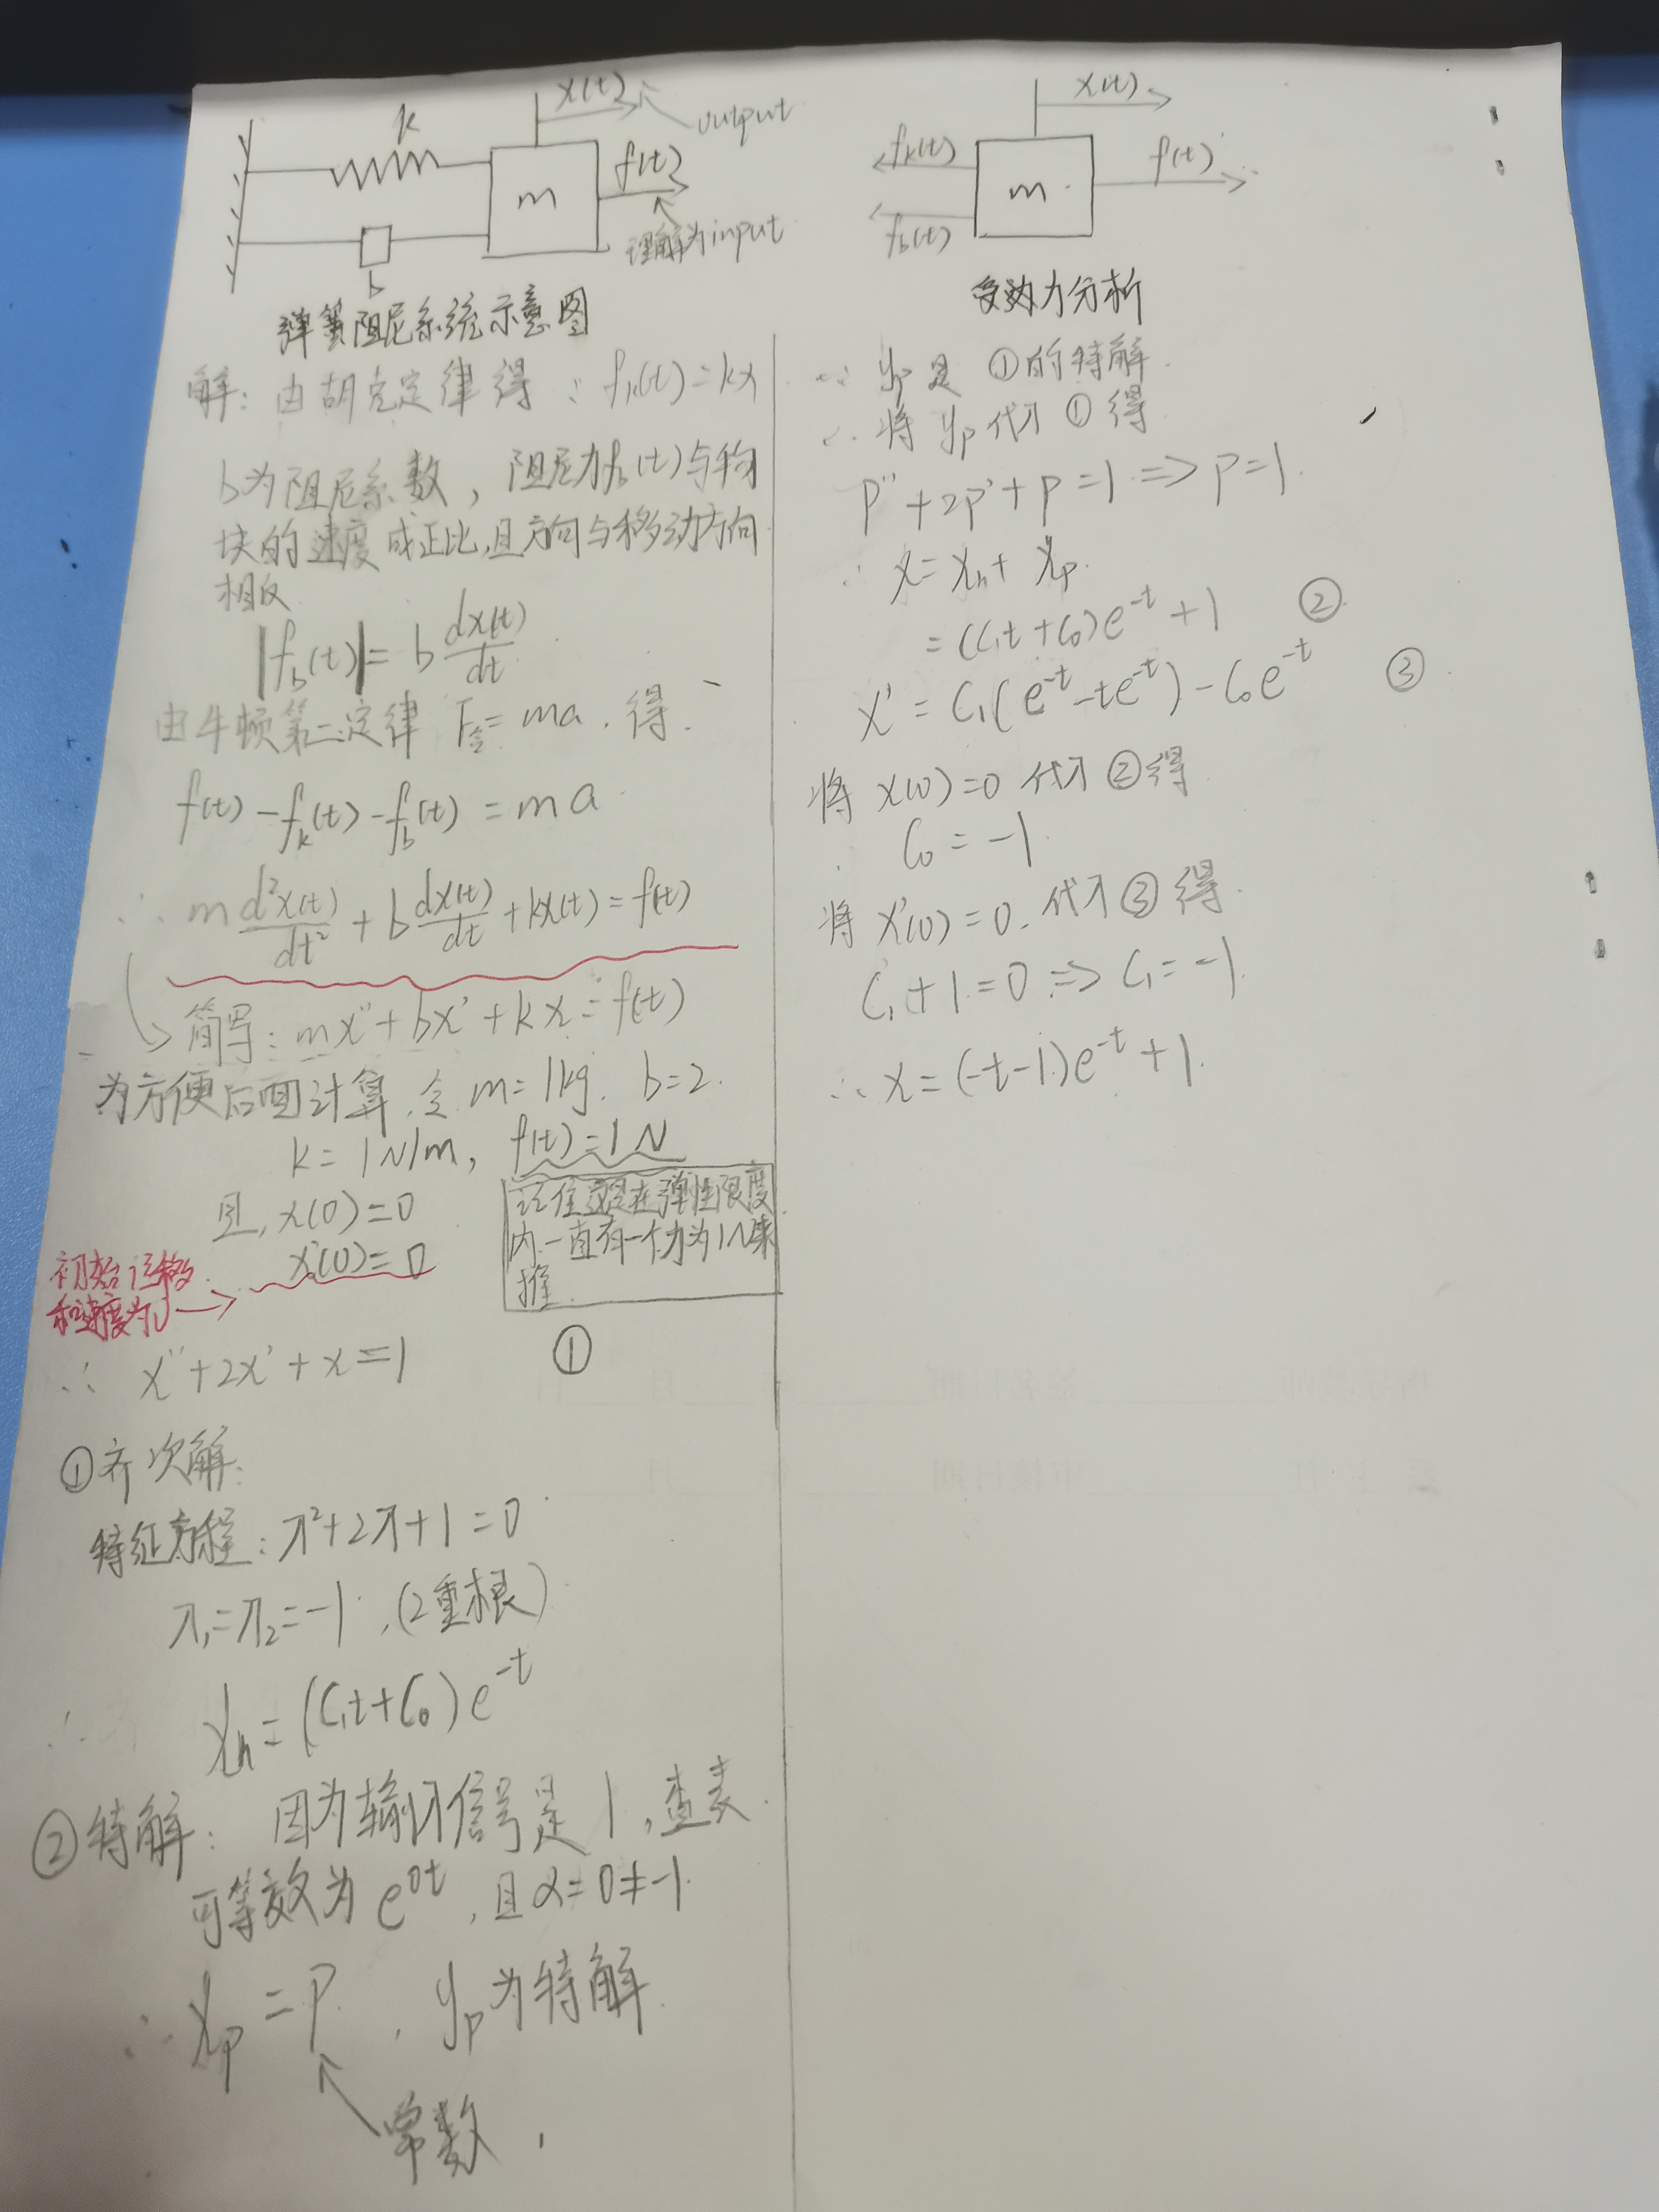
\includegraphics[width=10cm]{picture/spring_damper.png}
      \par 再看看最后计算的结果
      \par \includegraphics[width=10cm]{picture/result.png}
   \par 从图像看出,用恒定1N的力去推物块,他会在9s左右到达1m处,然后到达二力平衡,一直停在1m处,
   \par 建议大家试试在此系统上用不同的系数(改变b、m、k),不同的输入看看得到的结果是什么,自己算一遍会有不一样的收获。
    \end{notitlebox}
    \begin{flushleft}
      在现实生活中不一样的系统需要对应的系统建模方法,比如电路系统需要用KCL、KVL等,热力学需要PV=nRT、卡诺循环等。这些在你们需要的时候可以自行去探索,这里就不过多赘述了
    \end{flushleft}
  \subsection{卷积}
     \subsubsection{基本信号及其响应}
     \begin{flushleft}
      在讲卷积之前,我需要引入两个基本信号,以此来推导卷积的公式,同时这两个基本信号也非常重要,大家一定要熟悉。
     \end{flushleft}
     \begin{titlebox}{阶跃函数}
   
   $$ \varepsilon \left( t \right)=
      \begin{cases}
       0 \text{\hspace{0.5cm},t<0}\\
       1 \text{\hspace{0.5cm},t>0}
      \end{cases}$$
      \begin{center}
        \par \includegraphics[width=6cm]{picture/step_signal.png}
      \end{center}
     \end{titlebox}

    \begin{titlebox}{冲激函数}
      
      $$\varepsilon'(t)= \delta \left( t \right)=
      \begin{cases}
       0 \text{\hspace{0.5cm},$t\ne 0$}\\
       \int_{-\infty }^{+\infty } \delta(t) \, dt=1
      \end{cases}$$
      \begin{center}
        \par \includegraphics[width=6cm]{picture/deta_signal.png}
      \end{center}
      \begin{flushleft}
        $\delta(t)$ 是我们人为定义的一个函数,他是由$ \varepsilon (t)$求导可得。
        \par 可以理解为在$\delta(t)$冲激函数可以理解为一个在t=0 处无限高、无限窄,但面积为 1 的脉冲
      \end{flushleft}
       \par \textbf{冲激函数的性质:}
       \begin{itemize} 
        \item 取样性质: $\int_{-\infty }^{+\infty } \delta(t)\varphi(t)  \, dx=\varphi(0) $ {\scriptsize 可以自己想想为什么}  
        \item 缩放性:$\delta (at) =\dfrac{1}{|a|}  \delta ( t ) $
        \item 
        \item  
      \end{itemize}
    \end{titlebox}
      
  \begin{flushleft}
    \begin{titlebox}{什么是卷积}
      卷积的本质:信号的分解
    \end{titlebox}
  \end{flushleft}
  \subsection{拉普拉斯变化}


  \section{}

\end{document}

